% Created by tikzDevice version 0.12.6 on 2026-02-13 11:35:49
% !TEX encoding = UTF-8 Unicode
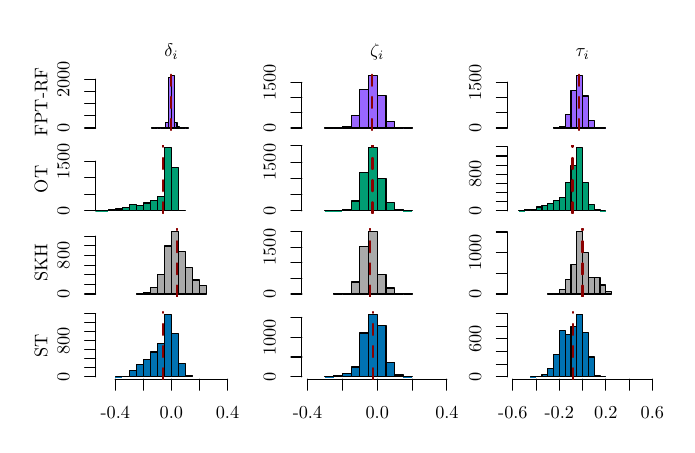
\begin{tikzpicture}[x=1pt,y=1pt]
\definecolor{fillColor}{RGB}{255,255,255}
\path[use as bounding box,fill=fillColor,fill opacity=0.00] (0,0) rectangle (230.90,143.67);
\begin{scope}
\path[clip] ( 24.55,106.66) rectangle ( 79.30,127.04);
\definecolor{drawColor}{RGB}{0,0,0}
\definecolor{fillColor}{RGB}{153,102,255}

\path[draw=drawColor,line width= 0.4pt,line join=round,line cap=round,fill=fillColor] ( 44.83,107.41) rectangle ( 45.84,107.42);

\path[draw=drawColor,line width= 0.4pt,line join=round,line cap=round,fill=fillColor] ( 45.84,107.41) rectangle ( 46.86,107.41);

\path[draw=drawColor,line width= 0.4pt,line join=round,line cap=round,fill=fillColor] ( 46.86,107.41) rectangle ( 47.87,107.48);

\path[draw=drawColor,line width= 0.4pt,line join=round,line cap=round,fill=fillColor] ( 47.87,107.41) rectangle ( 48.88,107.56);

\path[draw=drawColor,line width= 0.4pt,line join=round,line cap=round,fill=fillColor] ( 48.88,107.41) rectangle ( 49.90,107.72);

\path[draw=drawColor,line width= 0.4pt,line join=round,line cap=round,fill=fillColor] ( 49.90,107.41) rectangle ( 50.91,109.30);

\path[draw=drawColor,line width= 0.4pt,line join=round,line cap=round,fill=fillColor] ( 50.91,107.41) rectangle ( 51.92,125.75);

\path[draw=drawColor,line width= 0.4pt,line join=round,line cap=round,fill=fillColor] ( 51.92,107.41) rectangle ( 52.94,126.29);

\path[draw=drawColor,line width= 0.4pt,line join=round,line cap=round,fill=fillColor] ( 52.94,107.41) rectangle ( 53.95,109.34);

\path[draw=drawColor,line width= 0.4pt,line join=round,line cap=round,fill=fillColor] ( 53.95,107.41) rectangle ( 54.97,107.76);

\path[draw=drawColor,line width= 0.4pt,line join=round,line cap=round,fill=fillColor] ( 54.97,107.41) rectangle ( 55.98,107.51);

\path[draw=drawColor,line width= 0.4pt,line join=round,line cap=round,fill=fillColor] ( 55.98,107.41) rectangle ( 56.99,107.42);

\path[draw=drawColor,line width= 0.4pt,line join=round,line cap=round,fill=fillColor] ( 56.99,107.41) rectangle ( 58.01,107.42);
\end{scope}
\begin{scope}
\path[clip] (  0.00,  0.00) rectangle (230.90,143.67);
\definecolor{drawColor}{RGB}{0,0,0}

\path[draw=drawColor,line width= 0.4pt,line join=round,line cap=round] ( 24.55,107.41) -- ( 24.55,125.06);

\path[draw=drawColor,line width= 0.4pt,line join=round,line cap=round] ( 24.55,107.41) -- ( 20.59,107.41);

\path[draw=drawColor,line width= 0.4pt,line join=round,line cap=round] ( 24.55,111.83) -- ( 20.59,111.83);

\path[draw=drawColor,line width= 0.4pt,line join=round,line cap=round] ( 24.55,116.24) -- ( 20.59,116.24);

\path[draw=drawColor,line width= 0.4pt,line join=round,line cap=round] ( 24.55,120.65) -- ( 20.59,120.65);

\path[draw=drawColor,line width= 0.4pt,line join=round,line cap=round] ( 24.55,125.06) -- ( 20.59,125.06);

\node[text=drawColor,rotate= 90.00,anchor=base,inner sep=0pt, outer sep=0pt, scale=  0.66] at ( 15.05,107.41) {0};

\node[text=drawColor,rotate= 90.00,anchor=base,inner sep=0pt, outer sep=0pt, scale=  0.66] at ( 15.05,125.06) {2000};
\end{scope}
\begin{scope}
\path[clip] (  0.00,101.91) rectangle ( 82.47,143.67);
\definecolor{drawColor}{RGB}{0,0,0}

\node[text=drawColor,anchor=base,inner sep=0pt, outer sep=0pt, scale=  0.66] at ( 51.92,133.08) {\bfseries $\delta_i$};

\node[text=drawColor,rotate= 90.00,anchor=base,inner sep=0pt, outer sep=0pt, scale=  0.66] at (  7.13,116.85) {FPT-RF};
\end{scope}
\begin{scope}
\path[clip] ( 24.55,106.66) rectangle ( 79.30,127.04);
\definecolor{drawColor}{RGB}{139,0,0}

\path[draw=drawColor,line width= 0.8pt,dash pattern=on 4pt off 4pt ,line join=round,line cap=round] ( 51.93,106.66) -- ( 51.93,127.04);
\end{scope}
\begin{scope}
\path[clip] ( 99.10,106.66) rectangle (153.52,127.04);
\definecolor{drawColor}{RGB}{0,0,0}
\definecolor{fillColor}{RGB}{153,102,255}

\path[draw=drawColor,line width= 0.4pt,line join=round,line cap=round,fill=fillColor] (107.41,107.41) rectangle (110.56,107.43);

\path[draw=drawColor,line width= 0.4pt,line join=round,line cap=round,fill=fillColor] (110.56,107.41) rectangle (113.71,107.48);

\path[draw=drawColor,line width= 0.4pt,line join=round,line cap=round,fill=fillColor] (113.71,107.41) rectangle (116.86,107.87);

\path[draw=drawColor,line width= 0.4pt,line join=round,line cap=round,fill=fillColor] (116.86,107.41) rectangle (120.01,111.79);

\path[draw=drawColor,line width= 0.4pt,line join=round,line cap=round,fill=fillColor] (120.01,107.41) rectangle (123.16,121.29);

\path[draw=drawColor,line width= 0.4pt,line join=round,line cap=round,fill=fillColor] (123.16,107.41) rectangle (126.31,126.29);

\path[draw=drawColor,line width= 0.4pt,line join=round,line cap=round,fill=fillColor] (126.31,107.41) rectangle (129.46,119.09);

\path[draw=drawColor,line width= 0.4pt,line join=round,line cap=round,fill=fillColor] (129.46,107.41) rectangle (132.61,109.84);

\path[draw=drawColor,line width= 0.4pt,line join=round,line cap=round,fill=fillColor] (132.61,107.41) rectangle (135.75,107.73);

\path[draw=drawColor,line width= 0.4pt,line join=round,line cap=round,fill=fillColor] (135.75,107.41) rectangle (138.90,107.51);
\end{scope}
\begin{scope}
\path[clip] (  0.00,  0.00) rectangle (230.90,143.67);
\definecolor{drawColor}{RGB}{0,0,0}

\path[draw=drawColor,line width= 0.4pt,line join=round,line cap=round] ( 99.10,107.41) -- ( 99.10,123.85);

\path[draw=drawColor,line width= 0.4pt,line join=round,line cap=round] ( 99.10,107.41) -- ( 95.14,107.41);

\path[draw=drawColor,line width= 0.4pt,line join=round,line cap=round] ( 99.10,112.89) -- ( 95.14,112.89);

\path[draw=drawColor,line width= 0.4pt,line join=round,line cap=round] ( 99.10,118.37) -- ( 95.14,118.37);

\path[draw=drawColor,line width= 0.4pt,line join=round,line cap=round] ( 99.10,123.85) -- ( 95.14,123.85);

\node[text=drawColor,rotate= 90.00,anchor=base,inner sep=0pt, outer sep=0pt, scale=  0.66] at ( 89.59,107.41) {0};

\node[text=drawColor,rotate= 90.00,anchor=base,inner sep=0pt, outer sep=0pt, scale=  0.66] at ( 89.59,123.85) {1500};
\end{scope}
\begin{scope}
\path[clip] ( 82.47,101.91) rectangle (156.68,143.67);
\definecolor{drawColor}{RGB}{0,0,0}

\node[text=drawColor,anchor=base,inner sep=0pt, outer sep=0pt, scale=  0.66] at (126.31,133.08) {\bfseries $\zeta_i$};
\end{scope}
\begin{scope}
\path[clip] ( 99.10,106.66) rectangle (153.52,127.04);
\definecolor{drawColor}{RGB}{139,0,0}

\path[draw=drawColor,line width= 0.8pt,dash pattern=on 4pt off 4pt ,line join=round,line cap=round] (124.33,106.66) -- (124.33,127.04);
\end{scope}
\begin{scope}
\path[clip] (173.32,106.66) rectangle (227.73,127.04);
\definecolor{drawColor}{RGB}{0,0,0}
\definecolor{fillColor}{RGB}{153,102,255}

\path[draw=drawColor,line width= 0.4pt,line join=round,line cap=round,fill=fillColor] (190.03,107.41) rectangle (192.13,107.49);

\path[draw=drawColor,line width= 0.4pt,line join=round,line cap=round,fill=fillColor] (192.13,107.41) rectangle (194.23,107.91);

\path[draw=drawColor,line width= 0.4pt,line join=round,line cap=round,fill=fillColor] (194.23,107.41) rectangle (196.33,112.20);

\path[draw=drawColor,line width= 0.4pt,line join=round,line cap=round,fill=fillColor] (196.33,107.41) rectangle (198.43,121.12);

\path[draw=drawColor,line width= 0.4pt,line join=round,line cap=round,fill=fillColor] (198.43,107.41) rectangle (200.53,126.29);

\path[draw=drawColor,line width= 0.4pt,line join=round,line cap=round,fill=fillColor] (200.53,107.41) rectangle (202.62,118.99);

\path[draw=drawColor,line width= 0.4pt,line join=round,line cap=round,fill=fillColor] (202.62,107.41) rectangle (204.72,110.03);

\path[draw=drawColor,line width= 0.4pt,line join=round,line cap=round,fill=fillColor] (204.72,107.41) rectangle (206.82,107.75);

\path[draw=drawColor,line width= 0.4pt,line join=round,line cap=round,fill=fillColor] (206.82,107.41) rectangle (208.92,107.52);
\end{scope}
\begin{scope}
\path[clip] (  0.00,  0.00) rectangle (230.90,143.67);
\definecolor{drawColor}{RGB}{0,0,0}

\path[draw=drawColor,line width= 0.4pt,line join=round,line cap=round] (173.32,107.41) -- (173.32,123.98);

\path[draw=drawColor,line width= 0.4pt,line join=round,line cap=round] (173.32,107.41) -- (169.36,107.41);

\path[draw=drawColor,line width= 0.4pt,line join=round,line cap=round] (173.32,112.94) -- (169.36,112.94);

\path[draw=drawColor,line width= 0.4pt,line join=round,line cap=round] (173.32,118.46) -- (169.36,118.46);

\path[draw=drawColor,line width= 0.4pt,line join=round,line cap=round] (173.32,123.98) -- (169.36,123.98);

\node[text=drawColor,rotate= 90.00,anchor=base,inner sep=0pt, outer sep=0pt, scale=  0.66] at (163.81,107.41) {0};

\node[text=drawColor,rotate= 90.00,anchor=base,inner sep=0pt, outer sep=0pt, scale=  0.66] at (163.81,123.98) {1500};
\end{scope}
\begin{scope}
\path[clip] (156.68,101.91) rectangle (230.90,143.67);
\definecolor{drawColor}{RGB}{0,0,0}

\node[text=drawColor,anchor=base,inner sep=0pt, outer sep=0pt, scale=  0.66] at (200.53,133.08) {\bfseries $\tau_i$};
\end{scope}
\begin{scope}
\path[clip] (173.32,106.66) rectangle (227.73,127.04);
\definecolor{drawColor}{RGB}{139,0,0}

\path[draw=drawColor,line width= 0.8pt,dash pattern=on 4pt off 4pt ,line join=round,line cap=round] (199.21,106.66) -- (199.21,127.04);
\end{scope}
\begin{scope}
\path[clip] ( 24.55, 76.59) rectangle ( 79.30,101.12);
\definecolor{drawColor}{RGB}{0,0,0}
\definecolor{fillColor}{RGB}{0,158,115}

\path[draw=drawColor,line width= 0.4pt,line join=round,line cap=round,fill=fillColor] ( 24.05, 77.50) rectangle ( 26.58, 77.51);

\path[draw=drawColor,line width= 0.4pt,line join=round,line cap=round,fill=fillColor] ( 26.58, 77.50) rectangle ( 29.11, 77.58);

\path[draw=drawColor,line width= 0.4pt,line join=round,line cap=round,fill=fillColor] ( 29.11, 77.50) rectangle ( 31.65, 77.96);

\path[draw=drawColor,line width= 0.4pt,line join=round,line cap=round,fill=fillColor] ( 31.65, 77.50) rectangle ( 34.18, 78.15);

\path[draw=drawColor,line width= 0.4pt,line join=round,line cap=round,fill=fillColor] ( 34.18, 77.50) rectangle ( 36.72, 78.79);

\path[draw=drawColor,line width= 0.4pt,line join=round,line cap=round,fill=fillColor] ( 36.72, 77.50) rectangle ( 39.25, 79.63);

\path[draw=drawColor,line width= 0.4pt,line join=round,line cap=round,fill=fillColor] ( 39.25, 77.50) rectangle ( 41.79, 79.51);

\path[draw=drawColor,line width= 0.4pt,line join=round,line cap=round,fill=fillColor] ( 41.79, 77.50) rectangle ( 44.32, 80.33);

\path[draw=drawColor,line width= 0.4pt,line join=round,line cap=round,fill=fillColor] ( 44.32, 77.50) rectangle ( 46.86, 81.15);

\path[draw=drawColor,line width= 0.4pt,line join=round,line cap=round,fill=fillColor] ( 46.86, 77.50) rectangle ( 49.39, 82.70);

\path[draw=drawColor,line width= 0.4pt,line join=round,line cap=round,fill=fillColor] ( 49.39, 77.50) rectangle ( 51.92,100.21);

\path[draw=drawColor,line width= 0.4pt,line join=round,line cap=round,fill=fillColor] ( 51.92, 77.50) rectangle ( 54.46, 93.09);

\path[draw=drawColor,line width= 0.4pt,line join=round,line cap=round,fill=fillColor] ( 54.46, 77.50) rectangle ( 56.99, 77.68);
\end{scope}
\begin{scope}
\path[clip] (  0.00,  0.00) rectangle (230.90,143.67);
\definecolor{drawColor}{RGB}{0,0,0}

\path[draw=drawColor,line width= 0.4pt,line join=round,line cap=round] ( 24.55, 77.50) -- ( 24.55, 95.41);

\path[draw=drawColor,line width= 0.4pt,line join=round,line cap=round] ( 24.55, 77.50) -- ( 20.59, 77.50);

\path[draw=drawColor,line width= 0.4pt,line join=round,line cap=round] ( 24.55, 83.47) -- ( 20.59, 83.47);

\path[draw=drawColor,line width= 0.4pt,line join=round,line cap=round] ( 24.55, 89.44) -- ( 20.59, 89.44);

\path[draw=drawColor,line width= 0.4pt,line join=round,line cap=round] ( 24.55, 95.41) -- ( 20.59, 95.41);

\node[text=drawColor,rotate= 90.00,anchor=base,inner sep=0pt, outer sep=0pt, scale=  0.66] at ( 15.05, 77.50) {0};

\node[text=drawColor,rotate= 90.00,anchor=base,inner sep=0pt, outer sep=0pt, scale=  0.66] at ( 15.05, 95.41) {1500};
\end{scope}
\begin{scope}
\path[clip] (  0.00, 71.84) rectangle ( 82.47,101.91);
\definecolor{drawColor}{RGB}{0,0,0}

\node[text=drawColor,rotate= 90.00,anchor=base,inner sep=0pt, outer sep=0pt, scale=  0.66] at (  7.13, 88.85) {OT};
\end{scope}
\begin{scope}
\path[clip] ( 24.55, 76.59) rectangle ( 79.30,101.12);
\definecolor{drawColor}{RGB}{139,0,0}

\path[draw=drawColor,line width= 0.8pt,dash pattern=on 4pt off 4pt ,line join=round,line cap=round] ( 48.89, 76.59) -- ( 48.89,101.12);
\end{scope}
\begin{scope}
\path[clip] ( 99.10, 76.59) rectangle (153.52,101.12);
\definecolor{drawColor}{RGB}{0,0,0}
\definecolor{fillColor}{RGB}{0,158,115}

\path[draw=drawColor,line width= 0.4pt,line join=round,line cap=round,fill=fillColor] (107.41, 77.50) rectangle (110.56, 77.54);

\path[draw=drawColor,line width= 0.4pt,line join=round,line cap=round,fill=fillColor] (110.56, 77.50) rectangle (113.71, 77.53);

\path[draw=drawColor,line width= 0.4pt,line join=round,line cap=round,fill=fillColor] (113.71, 77.50) rectangle (116.86, 77.85);

\path[draw=drawColor,line width= 0.4pt,line join=round,line cap=round,fill=fillColor] (116.86, 77.50) rectangle (120.01, 81.02);

\path[draw=drawColor,line width= 0.4pt,line join=round,line cap=round,fill=fillColor] (120.01, 77.50) rectangle (123.16, 91.49);

\path[draw=drawColor,line width= 0.4pt,line join=round,line cap=round,fill=fillColor] (123.16, 77.50) rectangle (126.31,100.21);

\path[draw=drawColor,line width= 0.4pt,line join=round,line cap=round,fill=fillColor] (126.31, 77.50) rectangle (129.46, 89.19);

\path[draw=drawColor,line width= 0.4pt,line join=round,line cap=round,fill=fillColor] (129.46, 77.50) rectangle (132.61, 80.35);

\path[draw=drawColor,line width= 0.4pt,line join=round,line cap=round,fill=fillColor] (132.61, 77.50) rectangle (135.75, 78.07);

\path[draw=drawColor,line width= 0.4pt,line join=round,line cap=round,fill=fillColor] (135.75, 77.50) rectangle (138.90, 77.56);
\end{scope}
\begin{scope}
\path[clip] (  0.00,  0.00) rectangle (230.90,143.67);
\definecolor{drawColor}{RGB}{0,0,0}

\path[draw=drawColor,line width= 0.4pt,line join=round,line cap=round] ( 99.10, 77.50) -- ( 99.10,100.96);

\path[draw=drawColor,line width= 0.4pt,line join=round,line cap=round] ( 99.10, 77.50) -- ( 95.14, 77.50);

\path[draw=drawColor,line width= 0.4pt,line join=round,line cap=round] ( 99.10, 83.36) -- ( 95.14, 83.36);

\path[draw=drawColor,line width= 0.4pt,line join=round,line cap=round] ( 99.10, 89.23) -- ( 95.14, 89.23);

\path[draw=drawColor,line width= 0.4pt,line join=round,line cap=round] ( 99.10, 95.09) -- ( 95.14, 95.09);

\path[draw=drawColor,line width= 0.4pt,line join=round,line cap=round] ( 99.10,100.96) -- ( 95.14,100.96);

\node[text=drawColor,rotate= 90.00,anchor=base,inner sep=0pt, outer sep=0pt, scale=  0.66] at ( 89.59, 77.50) {0};

\node[text=drawColor,rotate= 90.00,anchor=base,inner sep=0pt, outer sep=0pt, scale=  0.66] at ( 89.59, 95.09) {1500};
\end{scope}
\begin{scope}
\path[clip] ( 99.10, 76.59) rectangle (153.52,101.12);
\definecolor{drawColor}{RGB}{139,0,0}

\path[draw=drawColor,line width= 0.8pt,dash pattern=on 4pt off 4pt ,line join=round,line cap=round] (124.60, 76.59) -- (124.60,101.12);
\end{scope}
\begin{scope}
\path[clip] (173.32, 76.59) rectangle (227.73,101.12);
\definecolor{drawColor}{RGB}{0,0,0}
\definecolor{fillColor}{RGB}{0,158,115}

\path[draw=drawColor,line width= 0.4pt,line join=round,line cap=round,fill=fillColor] (177.43, 77.50) rectangle (179.53, 77.58);

\path[draw=drawColor,line width= 0.4pt,line join=round,line cap=round,fill=fillColor] (179.53, 77.50) rectangle (181.63, 77.99);

\path[draw=drawColor,line width= 0.4pt,line join=round,line cap=round,fill=fillColor] (181.63, 77.50) rectangle (183.73, 78.12);

\path[draw=drawColor,line width= 0.4pt,line join=round,line cap=round,fill=fillColor] (183.73, 77.50) rectangle (185.83, 78.87);

\path[draw=drawColor,line width= 0.4pt,line join=round,line cap=round,fill=fillColor] (185.83, 77.50) rectangle (187.93, 79.57);

\path[draw=drawColor,line width= 0.4pt,line join=round,line cap=round,fill=fillColor] (187.93, 77.50) rectangle (190.03, 80.27);

\path[draw=drawColor,line width= 0.4pt,line join=round,line cap=round,fill=fillColor] (190.03, 77.50) rectangle (192.13, 81.36);

\path[draw=drawColor,line width= 0.4pt,line join=round,line cap=round,fill=fillColor] (192.13, 77.50) rectangle (194.23, 82.44);

\path[draw=drawColor,line width= 0.4pt,line join=round,line cap=round,fill=fillColor] (194.23, 77.50) rectangle (196.33, 87.71);

\path[draw=drawColor,line width= 0.4pt,line join=round,line cap=round,fill=fillColor] (196.33, 77.50) rectangle (198.43, 94.02);

\path[draw=drawColor,line width= 0.4pt,line join=round,line cap=round,fill=fillColor] (198.43, 77.50) rectangle (200.53,100.21);

\path[draw=drawColor,line width= 0.4pt,line join=round,line cap=round,fill=fillColor] (200.53, 77.50) rectangle (202.62, 87.66);

\path[draw=drawColor,line width= 0.4pt,line join=round,line cap=round,fill=fillColor] (202.62, 77.50) rectangle (204.72, 79.81);

\path[draw=drawColor,line width= 0.4pt,line join=round,line cap=round,fill=fillColor] (204.72, 77.50) rectangle (206.82, 77.84);

\path[draw=drawColor,line width= 0.4pt,line join=round,line cap=round,fill=fillColor] (206.82, 77.50) rectangle (208.92, 77.51);
\end{scope}
\begin{scope}
\path[clip] (  0.00,  0.00) rectangle (230.90,143.67);
\definecolor{drawColor}{RGB}{0,0,0}

\path[draw=drawColor,line width= 0.4pt,line join=round,line cap=round] (173.32, 77.50) -- (173.32,100.59);

\path[draw=drawColor,line width= 0.4pt,line join=round,line cap=round] (173.32, 77.50) -- (169.36, 77.50);

\path[draw=drawColor,line width= 0.4pt,line join=round,line cap=round] (173.32, 80.80) -- (169.36, 80.80);

\path[draw=drawColor,line width= 0.4pt,line join=round,line cap=round] (173.32, 84.09) -- (169.36, 84.09);

\path[draw=drawColor,line width= 0.4pt,line join=round,line cap=round] (173.32, 87.39) -- (169.36, 87.39);

\path[draw=drawColor,line width= 0.4pt,line join=round,line cap=round] (173.32, 90.69) -- (169.36, 90.69);

\path[draw=drawColor,line width= 0.4pt,line join=round,line cap=round] (173.32, 93.99) -- (169.36, 93.99);

\path[draw=drawColor,line width= 0.4pt,line join=round,line cap=round] (173.32, 97.29) -- (169.36, 97.29);

\path[draw=drawColor,line width= 0.4pt,line join=round,line cap=round] (173.32,100.59) -- (169.36,100.59);

\node[text=drawColor,rotate= 90.00,anchor=base,inner sep=0pt, outer sep=0pt, scale=  0.66] at (163.81, 77.50) {0};

\node[text=drawColor,rotate= 90.00,anchor=base,inner sep=0pt, outer sep=0pt, scale=  0.66] at (163.81, 90.69) {800};
\end{scope}
\begin{scope}
\path[clip] (173.32, 76.59) rectangle (227.73,101.12);
\definecolor{drawColor}{RGB}{139,0,0}

\path[draw=drawColor,line width= 0.8pt,dash pattern=on 4pt off 4pt ,line join=round,line cap=round] (196.87, 76.59) -- (196.87,101.12);
\end{scope}
\begin{scope}
\path[clip] ( 24.55, 46.52) rectangle ( 79.30, 71.04);
\definecolor{drawColor}{RGB}{0,0,0}
\definecolor{fillColor}{RGB}{169,169,169}

\path[draw=drawColor,line width= 0.4pt,line join=round,line cap=round,fill=fillColor] ( 39.25, 47.43) rectangle ( 41.79, 47.44);

\path[draw=drawColor,line width= 0.4pt,line join=round,line cap=round,fill=fillColor] ( 41.79, 47.43) rectangle ( 44.32, 47.90);

\path[draw=drawColor,line width= 0.4pt,line join=round,line cap=round,fill=fillColor] ( 44.32, 47.43) rectangle ( 46.86, 49.74);

\path[draw=drawColor,line width= 0.4pt,line join=round,line cap=round,fill=fillColor] ( 46.86, 47.43) rectangle ( 49.39, 54.50);

\path[draw=drawColor,line width= 0.4pt,line join=round,line cap=round,fill=fillColor] ( 49.39, 47.43) rectangle ( 51.92, 64.77);

\path[draw=drawColor,line width= 0.4pt,line join=round,line cap=round,fill=fillColor] ( 51.92, 47.43) rectangle ( 54.46, 70.14);

\path[draw=drawColor,line width= 0.4pt,line join=round,line cap=round,fill=fillColor] ( 54.46, 47.43) rectangle ( 56.99, 62.64);

\path[draw=drawColor,line width= 0.4pt,line join=round,line cap=round,fill=fillColor] ( 56.99, 47.43) rectangle ( 59.53, 57.06);

\path[draw=drawColor,line width= 0.4pt,line join=round,line cap=round,fill=fillColor] ( 59.53, 47.43) rectangle ( 62.06, 52.50);

\path[draw=drawColor,line width= 0.4pt,line join=round,line cap=round,fill=fillColor] ( 62.06, 47.43) rectangle ( 64.60, 50.53);
\end{scope}
\begin{scope}
\path[clip] (  0.00,  0.00) rectangle (230.90,143.67);
\definecolor{drawColor}{RGB}{0,0,0}

\path[draw=drawColor,line width= 0.4pt,line join=round,line cap=round] ( 24.55, 47.43) -- ( 24.55, 68.34);

\path[draw=drawColor,line width= 0.4pt,line join=round,line cap=round] ( 24.55, 47.43) -- ( 20.59, 47.43);

\path[draw=drawColor,line width= 0.4pt,line join=round,line cap=round] ( 24.55, 50.91) -- ( 20.59, 50.91);

\path[draw=drawColor,line width= 0.4pt,line join=round,line cap=round] ( 24.55, 54.40) -- ( 20.59, 54.40);

\path[draw=drawColor,line width= 0.4pt,line join=round,line cap=round] ( 24.55, 57.88) -- ( 20.59, 57.88);

\path[draw=drawColor,line width= 0.4pt,line join=round,line cap=round] ( 24.55, 61.37) -- ( 20.59, 61.37);

\path[draw=drawColor,line width= 0.4pt,line join=round,line cap=round] ( 24.55, 64.85) -- ( 20.59, 64.85);

\path[draw=drawColor,line width= 0.4pt,line join=round,line cap=round] ( 24.55, 68.34) -- ( 20.59, 68.34);

\node[text=drawColor,rotate= 90.00,anchor=base,inner sep=0pt, outer sep=0pt, scale=  0.66] at ( 15.05, 47.43) {0};

\node[text=drawColor,rotate= 90.00,anchor=base,inner sep=0pt, outer sep=0pt, scale=  0.66] at ( 15.05, 61.37) {800};
\end{scope}
\begin{scope}
\path[clip] (  0.00, 41.77) rectangle ( 82.47, 71.84);
\definecolor{drawColor}{RGB}{0,0,0}

\node[text=drawColor,rotate= 90.00,anchor=base,inner sep=0pt, outer sep=0pt, scale=  0.66] at (  7.13, 58.78) {SKH};
\end{scope}
\begin{scope}
\path[clip] ( 24.55, 46.52) rectangle ( 79.30, 71.04);
\definecolor{drawColor}{RGB}{139,0,0}

\path[draw=drawColor,line width= 0.8pt,dash pattern=on 4pt off 4pt ,line join=round,line cap=round] ( 53.87, 46.52) -- ( 53.87, 71.04);
\end{scope}
\begin{scope}
\path[clip] ( 99.10, 46.52) rectangle (153.52, 71.04);
\definecolor{drawColor}{RGB}{0,0,0}
\definecolor{fillColor}{RGB}{169,169,169}

\path[draw=drawColor,line width= 0.4pt,line join=round,line cap=round,fill=fillColor] (110.56, 47.43) rectangle (113.71, 47.48);

\path[draw=drawColor,line width= 0.4pt,line join=round,line cap=round,fill=fillColor] (113.71, 47.43) rectangle (116.86, 47.60);

\path[draw=drawColor,line width= 0.4pt,line join=round,line cap=round,fill=fillColor] (116.86, 47.43) rectangle (120.01, 51.78);

\path[draw=drawColor,line width= 0.4pt,line join=round,line cap=round,fill=fillColor] (120.01, 47.43) rectangle (123.16, 64.65);

\path[draw=drawColor,line width= 0.4pt,line join=round,line cap=round,fill=fillColor] (123.16, 47.43) rectangle (126.31, 70.14);

\path[draw=drawColor,line width= 0.4pt,line join=round,line cap=round,fill=fillColor] (126.31, 47.43) rectangle (129.46, 54.33);

\path[draw=drawColor,line width= 0.4pt,line join=round,line cap=round,fill=fillColor] (129.46, 47.43) rectangle (132.61, 49.61);

\path[draw=drawColor,line width= 0.4pt,line join=round,line cap=round,fill=fillColor] (132.61, 47.43) rectangle (135.75, 47.54);

\path[draw=drawColor,line width= 0.4pt,line join=round,line cap=round,fill=fillColor] (135.75, 47.43) rectangle (138.90, 47.52);
\end{scope}
\begin{scope}
\path[clip] (  0.00,  0.00) rectangle (230.90,143.67);
\definecolor{drawColor}{RGB}{0,0,0}

\path[draw=drawColor,line width= 0.4pt,line join=round,line cap=round] ( 99.10, 47.43) -- ( 99.10, 70.03);

\path[draw=drawColor,line width= 0.4pt,line join=round,line cap=round] ( 99.10, 47.43) -- ( 95.14, 47.43);

\path[draw=drawColor,line width= 0.4pt,line join=round,line cap=round] ( 99.10, 53.08) -- ( 95.14, 53.08);

\path[draw=drawColor,line width= 0.4pt,line join=round,line cap=round] ( 99.10, 58.73) -- ( 95.14, 58.73);

\path[draw=drawColor,line width= 0.4pt,line join=round,line cap=round] ( 99.10, 64.38) -- ( 95.14, 64.38);

\path[draw=drawColor,line width= 0.4pt,line join=round,line cap=round] ( 99.10, 70.03) -- ( 95.14, 70.03);

\node[text=drawColor,rotate= 90.00,anchor=base,inner sep=0pt, outer sep=0pt, scale=  0.66] at ( 89.59, 47.43) {0};

\node[text=drawColor,rotate= 90.00,anchor=base,inner sep=0pt, outer sep=0pt, scale=  0.66] at ( 89.59, 64.38) {1500};
\end{scope}
\begin{scope}
\path[clip] ( 99.10, 46.52) rectangle (153.52, 71.04);
\definecolor{drawColor}{RGB}{139,0,0}

\path[draw=drawColor,line width= 0.8pt,dash pattern=on 4pt off 4pt ,line join=round,line cap=round] (123.83, 46.52) -- (123.83, 71.04);
\end{scope}
\begin{scope}
\path[clip] (173.32, 46.52) rectangle (227.73, 71.04);
\definecolor{drawColor}{RGB}{0,0,0}
\definecolor{fillColor}{RGB}{169,169,169}

\path[draw=drawColor,line width= 0.4pt,line join=round,line cap=round,fill=fillColor] (187.93, 47.43) rectangle (190.03, 47.44);

\path[draw=drawColor,line width= 0.4pt,line join=round,line cap=round,fill=fillColor] (190.03, 47.43) rectangle (192.13, 47.61);

\path[draw=drawColor,line width= 0.4pt,line join=round,line cap=round,fill=fillColor] (192.13, 47.43) rectangle (194.23, 48.99);

\path[draw=drawColor,line width= 0.4pt,line join=round,line cap=round,fill=fillColor] (194.23, 47.43) rectangle (196.33, 52.68);

\path[draw=drawColor,line width= 0.4pt,line join=round,line cap=round,fill=fillColor] (196.33, 47.43) rectangle (198.43, 57.94);

\path[draw=drawColor,line width= 0.4pt,line join=round,line cap=round,fill=fillColor] (198.43, 47.43) rectangle (200.53, 70.14);

\path[draw=drawColor,line width= 0.4pt,line join=round,line cap=round,fill=fillColor] (200.53, 47.43) rectangle (202.62, 62.34);

\path[draw=drawColor,line width= 0.4pt,line join=round,line cap=round,fill=fillColor] (202.62, 47.43) rectangle (204.72, 53.36);

\path[draw=drawColor,line width= 0.4pt,line join=round,line cap=round,fill=fillColor] (204.72, 47.43) rectangle (206.82, 53.28);

\path[draw=drawColor,line width= 0.4pt,line join=round,line cap=round,fill=fillColor] (206.82, 47.43) rectangle (208.92, 50.70);

\path[draw=drawColor,line width= 0.4pt,line join=round,line cap=round,fill=fillColor] (208.92, 47.43) rectangle (211.02, 48.32);
\end{scope}
\begin{scope}
\path[clip] (  0.00,  0.00) rectangle (230.90,143.67);
\definecolor{drawColor}{RGB}{0,0,0}

\path[draw=drawColor,line width= 0.4pt,line join=round,line cap=round] (173.32, 47.43) -- (173.32, 69.84);

\path[draw=drawColor,line width= 0.4pt,line join=round,line cap=round] (173.32, 47.43) -- (169.36, 47.43);

\path[draw=drawColor,line width= 0.4pt,line join=round,line cap=round] (173.32, 54.90) -- (169.36, 54.90);

\path[draw=drawColor,line width= 0.4pt,line join=round,line cap=round] (173.32, 62.37) -- (169.36, 62.37);

\path[draw=drawColor,line width= 0.4pt,line join=round,line cap=round] (173.32, 69.84) -- (169.36, 69.84);

\node[text=drawColor,rotate= 90.00,anchor=base,inner sep=0pt, outer sep=0pt, scale=  0.66] at (163.81, 47.43) {0};

\node[text=drawColor,rotate= 90.00,anchor=base,inner sep=0pt, outer sep=0pt, scale=  0.66] at (163.81, 62.37) {1000};
\end{scope}
\begin{scope}
\path[clip] (173.32, 46.52) rectangle (227.73, 71.04);
\definecolor{drawColor}{RGB}{139,0,0}

\path[draw=drawColor,line width= 0.8pt,dash pattern=on 4pt off 4pt ,line join=round,line cap=round] (200.49, 46.52) -- (200.49, 71.04);
\end{scope}
\begin{scope}
\path[clip] ( 24.55, 16.63) rectangle ( 79.30, 40.97);
\definecolor{drawColor}{RGB}{0,0,0}
\definecolor{fillColor}{RGB}{0,114,178}

\path[draw=drawColor,line width= 0.4pt,line join=round,line cap=round,fill=fillColor] ( 31.65, 17.53) rectangle ( 34.18, 17.55);

\path[draw=drawColor,line width= 0.4pt,line join=round,line cap=round,fill=fillColor] ( 34.18, 17.53) rectangle ( 36.72, 17.73);

\path[draw=drawColor,line width= 0.4pt,line join=round,line cap=round,fill=fillColor] ( 36.72, 17.53) rectangle ( 39.25, 19.70);

\path[draw=drawColor,line width= 0.4pt,line join=round,line cap=round,fill=fillColor] ( 39.25, 17.53) rectangle ( 41.79, 21.89);

\path[draw=drawColor,line width= 0.4pt,line join=round,line cap=round,fill=fillColor] ( 41.79, 17.53) rectangle ( 44.32, 23.70);

\path[draw=drawColor,line width= 0.4pt,line join=round,line cap=round,fill=fillColor] ( 44.32, 17.53) rectangle ( 46.86, 26.49);

\path[draw=drawColor,line width= 0.4pt,line join=round,line cap=round,fill=fillColor] ( 46.86, 17.53) rectangle ( 49.39, 29.47);

\path[draw=drawColor,line width= 0.4pt,line join=round,line cap=round,fill=fillColor] ( 49.39, 17.53) rectangle ( 51.92, 40.07);

\path[draw=drawColor,line width= 0.4pt,line join=round,line cap=round,fill=fillColor] ( 51.92, 17.53) rectangle ( 54.46, 33.21);

\path[draw=drawColor,line width= 0.4pt,line join=round,line cap=round,fill=fillColor] ( 54.46, 17.53) rectangle ( 56.99, 22.35);

\path[draw=drawColor,line width= 0.4pt,line join=round,line cap=round,fill=fillColor] ( 56.99, 17.53) rectangle ( 59.53, 18.12);
\end{scope}
\begin{scope}
\path[clip] (  0.00,  0.00) rectangle (230.90,143.67);
\definecolor{drawColor}{RGB}{0,0,0}

\path[draw=drawColor,line width= 0.4pt,line join=round,line cap=round] ( 31.65, 16.63) -- ( 72.20, 16.63);

\path[draw=drawColor,line width= 0.4pt,line join=round,line cap=round] ( 31.65, 16.63) -- ( 31.65, 12.67);

\path[draw=drawColor,line width= 0.4pt,line join=round,line cap=round] ( 41.79, 16.63) -- ( 41.79, 12.67);

\path[draw=drawColor,line width= 0.4pt,line join=round,line cap=round] ( 51.92, 16.63) -- ( 51.92, 12.67);

\path[draw=drawColor,line width= 0.4pt,line join=round,line cap=round] ( 62.06, 16.63) -- ( 62.06, 12.67);

\path[draw=drawColor,line width= 0.4pt,line join=round,line cap=round] ( 72.20, 16.63) -- ( 72.20, 12.67);

\node[text=drawColor,anchor=base,inner sep=0pt, outer sep=0pt, scale=  0.66] at ( 31.65,  2.38) {-0.4};

\node[text=drawColor,anchor=base,inner sep=0pt, outer sep=0pt, scale=  0.66] at ( 51.92,  2.38) {0.0};

\node[text=drawColor,anchor=base,inner sep=0pt, outer sep=0pt, scale=  0.66] at ( 72.20,  2.38) {0.4};

\path[draw=drawColor,line width= 0.4pt,line join=round,line cap=round] ( 24.55, 17.53) -- ( 24.55, 40.30);

\path[draw=drawColor,line width= 0.4pt,line join=round,line cap=round] ( 24.55, 17.53) -- ( 20.59, 17.53);

\path[draw=drawColor,line width= 0.4pt,line join=round,line cap=round] ( 24.55, 20.79) -- ( 20.59, 20.79);

\path[draw=drawColor,line width= 0.4pt,line join=round,line cap=round] ( 24.55, 24.04) -- ( 20.59, 24.04);

\path[draw=drawColor,line width= 0.4pt,line join=round,line cap=round] ( 24.55, 27.29) -- ( 20.59, 27.29);

\path[draw=drawColor,line width= 0.4pt,line join=round,line cap=round] ( 24.55, 30.54) -- ( 20.59, 30.54);

\path[draw=drawColor,line width= 0.4pt,line join=round,line cap=round] ( 24.55, 33.79) -- ( 20.59, 33.79);

\path[draw=drawColor,line width= 0.4pt,line join=round,line cap=round] ( 24.55, 37.05) -- ( 20.59, 37.05);

\path[draw=drawColor,line width= 0.4pt,line join=round,line cap=round] ( 24.55, 40.30) -- ( 20.59, 40.30);

\node[text=drawColor,rotate= 90.00,anchor=base,inner sep=0pt, outer sep=0pt, scale=  0.66] at ( 15.05, 17.53) {0};

\node[text=drawColor,rotate= 90.00,anchor=base,inner sep=0pt, outer sep=0pt, scale=  0.66] at ( 15.05, 30.54) {800};
\end{scope}
\begin{scope}
\path[clip] (  0.00,  0.00) rectangle ( 82.47, 41.77);
\definecolor{drawColor}{RGB}{0,0,0}

\node[text=drawColor,rotate= 90.00,anchor=base,inner sep=0pt, outer sep=0pt, scale=  0.66] at (  7.13, 28.80) {ST};
\end{scope}
\begin{scope}
\path[clip] ( 24.55, 16.63) rectangle ( 79.30, 40.97);
\definecolor{drawColor}{RGB}{139,0,0}

\path[draw=drawColor,line width= 0.8pt,dash pattern=on 4pt off 4pt ,line join=round,line cap=round] ( 49.01, 16.63) -- ( 49.01, 40.97);
\end{scope}
\begin{scope}
\path[clip] ( 99.10, 16.63) rectangle (153.52, 40.97);
\definecolor{drawColor}{RGB}{0,0,0}
\definecolor{fillColor}{RGB}{0,114,178}

\path[draw=drawColor,line width= 0.4pt,line join=round,line cap=round,fill=fillColor] (107.41, 17.53) rectangle (110.56, 17.59);

\path[draw=drawColor,line width= 0.4pt,line join=round,line cap=round,fill=fillColor] (110.56, 17.53) rectangle (113.71, 17.83);

\path[draw=drawColor,line width= 0.4pt,line join=round,line cap=round,fill=fillColor] (113.71, 17.53) rectangle (116.86, 18.69);

\path[draw=drawColor,line width= 0.4pt,line join=round,line cap=round,fill=fillColor] (116.86, 17.53) rectangle (120.01, 21.06);

\path[draw=drawColor,line width= 0.4pt,line join=round,line cap=round,fill=fillColor] (120.01, 17.53) rectangle (123.16, 33.33);

\path[draw=drawColor,line width= 0.4pt,line join=round,line cap=round,fill=fillColor] (123.16, 17.53) rectangle (126.31, 40.07);

\path[draw=drawColor,line width= 0.4pt,line join=round,line cap=round,fill=fillColor] (126.31, 17.53) rectangle (129.46, 36.20);

\path[draw=drawColor,line width= 0.4pt,line join=round,line cap=round,fill=fillColor] (129.46, 17.53) rectangle (132.61, 22.84);

\path[draw=drawColor,line width= 0.4pt,line join=round,line cap=round,fill=fillColor] (132.61, 17.53) rectangle (135.75, 18.15);

\path[draw=drawColor,line width= 0.4pt,line join=round,line cap=round,fill=fillColor] (135.75, 17.53) rectangle (138.90, 17.60);
\end{scope}
\begin{scope}
\path[clip] (  0.00,  0.00) rectangle (230.90,143.67);
\definecolor{drawColor}{RGB}{0,0,0}

\path[draw=drawColor,line width= 0.4pt,line join=round,line cap=round] (101.11, 16.63) -- (151.50, 16.63);

\path[draw=drawColor,line width= 0.4pt,line join=round,line cap=round] (101.11, 16.63) -- (101.11, 12.67);

\path[draw=drawColor,line width= 0.4pt,line join=round,line cap=round] (113.71, 16.63) -- (113.71, 12.67);

\path[draw=drawColor,line width= 0.4pt,line join=round,line cap=round] (126.31, 16.63) -- (126.31, 12.67);

\path[draw=drawColor,line width= 0.4pt,line join=round,line cap=round] (138.90, 16.63) -- (138.90, 12.67);

\path[draw=drawColor,line width= 0.4pt,line join=round,line cap=round] (151.50, 16.63) -- (151.50, 12.67);

\node[text=drawColor,anchor=base,inner sep=0pt, outer sep=0pt, scale=  0.66] at (101.11,  2.38) {-0.4};

\node[text=drawColor,anchor=base,inner sep=0pt, outer sep=0pt, scale=  0.66] at (126.31,  2.38) {0.0};

\node[text=drawColor,anchor=base,inner sep=0pt, outer sep=0pt, scale=  0.66] at (151.50,  2.38) {0.4};

\path[draw=drawColor,line width= 0.4pt,line join=round,line cap=round] ( 99.10, 17.53) -- ( 99.10, 38.97);

\path[draw=drawColor,line width= 0.4pt,line join=round,line cap=round] ( 99.10, 17.53) -- ( 95.14, 17.53);

\path[draw=drawColor,line width= 0.4pt,line join=round,line cap=round] ( 99.10, 24.68) -- ( 95.14, 24.68);

\path[draw=drawColor,line width= 0.4pt,line join=round,line cap=round] ( 99.10, 31.83) -- ( 95.14, 31.83);

\path[draw=drawColor,line width= 0.4pt,line join=round,line cap=round] ( 99.10, 38.97) -- ( 95.14, 38.97);

\node[text=drawColor,rotate= 90.00,anchor=base,inner sep=0pt, outer sep=0pt, scale=  0.66] at ( 89.59, 17.53) {0};

\node[text=drawColor,rotate= 90.00,anchor=base,inner sep=0pt, outer sep=0pt, scale=  0.66] at ( 89.59, 31.83) {1000};
\end{scope}
\begin{scope}
\path[clip] ( 99.10, 16.63) rectangle (153.52, 40.97);
\definecolor{drawColor}{RGB}{139,0,0}

\path[draw=drawColor,line width= 0.8pt,dash pattern=on 4pt off 4pt ,line join=round,line cap=round] (124.86, 16.63) -- (124.86, 40.97);
\end{scope}
\begin{scope}
\path[clip] (173.32, 16.63) rectangle (227.73, 40.97);
\definecolor{drawColor}{RGB}{0,0,0}
\definecolor{fillColor}{RGB}{0,114,178}

\path[draw=drawColor,line width= 0.4pt,line join=round,line cap=round,fill=fillColor] (181.63, 17.53) rectangle (183.73, 17.58);

\path[draw=drawColor,line width= 0.4pt,line join=round,line cap=round,fill=fillColor] (183.73, 17.53) rectangle (185.83, 17.76);

\path[draw=drawColor,line width= 0.4pt,line join=round,line cap=round,fill=fillColor] (185.83, 17.53) rectangle (187.93, 18.31);

\path[draw=drawColor,line width= 0.4pt,line join=round,line cap=round,fill=fillColor] (187.93, 17.53) rectangle (190.03, 20.63);

\path[draw=drawColor,line width= 0.4pt,line join=round,line cap=round,fill=fillColor] (190.03, 17.53) rectangle (192.13, 25.44);

\path[draw=drawColor,line width= 0.4pt,line join=round,line cap=round,fill=fillColor] (192.13, 17.53) rectangle (194.23, 34.12);

\path[draw=drawColor,line width= 0.4pt,line join=round,line cap=round,fill=fillColor] (194.23, 17.53) rectangle (196.33, 32.85);

\path[draw=drawColor,line width= 0.4pt,line join=round,line cap=round,fill=fillColor] (196.33, 17.53) rectangle (198.43, 35.70);

\path[draw=drawColor,line width= 0.4pt,line join=round,line cap=round,fill=fillColor] (198.43, 17.53) rectangle (200.53, 40.07);

\path[draw=drawColor,line width= 0.4pt,line join=round,line cap=round,fill=fillColor] (200.53, 17.53) rectangle (202.62, 33.55);

\path[draw=drawColor,line width= 0.4pt,line join=round,line cap=round,fill=fillColor] (202.62, 17.53) rectangle (204.72, 24.67);

\path[draw=drawColor,line width= 0.4pt,line join=round,line cap=round,fill=fillColor] (204.72, 17.53) rectangle (206.82, 18.08);

\path[draw=drawColor,line width= 0.4pt,line join=round,line cap=round,fill=fillColor] (206.82, 17.53) rectangle (208.92, 17.65);
\end{scope}
\begin{scope}
\path[clip] (  0.00,  0.00) rectangle (230.90,143.67);
\definecolor{drawColor}{RGB}{0,0,0}

\path[draw=drawColor,line width= 0.4pt,line join=round,line cap=round] (175.33, 16.63) -- (225.72, 16.63);

\path[draw=drawColor,line width= 0.4pt,line join=round,line cap=round] (175.33, 16.63) -- (175.33, 12.67);

\path[draw=drawColor,line width= 0.4pt,line join=round,line cap=round] (183.73, 16.63) -- (183.73, 12.67);

\path[draw=drawColor,line width= 0.4pt,line join=round,line cap=round] (192.13, 16.63) -- (192.13, 12.67);

\path[draw=drawColor,line width= 0.4pt,line join=round,line cap=round] (200.53, 16.63) -- (200.53, 12.67);

\path[draw=drawColor,line width= 0.4pt,line join=round,line cap=round] (208.92, 16.63) -- (208.92, 12.67);

\path[draw=drawColor,line width= 0.4pt,line join=round,line cap=round] (217.32, 16.63) -- (217.32, 12.67);

\path[draw=drawColor,line width= 0.4pt,line join=round,line cap=round] (225.72, 16.63) -- (225.72, 12.67);

\node[text=drawColor,anchor=base,inner sep=0pt, outer sep=0pt, scale=  0.66] at (175.33,  2.38) {-0.6};

\node[text=drawColor,anchor=base,inner sep=0pt, outer sep=0pt, scale=  0.66] at (192.13,  2.38) {-0.2};

\node[text=drawColor,anchor=base,inner sep=0pt, outer sep=0pt, scale=  0.66] at (208.92,  2.38) {0.2};

\node[text=drawColor,anchor=base,inner sep=0pt, outer sep=0pt, scale=  0.66] at (225.72,  2.38) {0.6};

\path[draw=drawColor,line width= 0.4pt,line join=round,line cap=round] (173.32, 17.53) -- (173.32, 40.32);

\path[draw=drawColor,line width= 0.4pt,line join=round,line cap=round] (173.32, 17.53) -- (169.36, 17.53);

\path[draw=drawColor,line width= 0.4pt,line join=round,line cap=round] (173.32, 22.09) -- (169.36, 22.09);

\path[draw=drawColor,line width= 0.4pt,line join=round,line cap=round] (173.32, 26.65) -- (169.36, 26.65);

\path[draw=drawColor,line width= 0.4pt,line join=round,line cap=round] (173.32, 31.21) -- (169.36, 31.21);

\path[draw=drawColor,line width= 0.4pt,line join=round,line cap=round] (173.32, 35.76) -- (169.36, 35.76);

\path[draw=drawColor,line width= 0.4pt,line join=round,line cap=round] (173.32, 40.32) -- (169.36, 40.32);

\node[text=drawColor,rotate= 90.00,anchor=base,inner sep=0pt, outer sep=0pt, scale=  0.66] at (163.81, 17.53) {0};

\node[text=drawColor,rotate= 90.00,anchor=base,inner sep=0pt, outer sep=0pt, scale=  0.66] at (163.81, 31.21) {600};
\end{scope}
\begin{scope}
\path[clip] (173.32, 16.63) rectangle (227.73, 40.97);
\definecolor{drawColor}{RGB}{139,0,0}

\path[draw=drawColor,line width= 0.8pt,dash pattern=on 4pt off 4pt ,line join=round,line cap=round] (197.15, 16.63) -- (197.15, 40.97);
\end{scope}
\end{tikzpicture}
